\section[Design 2]{Design 2}
% Første parameter i [] er tekst i header. {} er i indholdsfortegnelsen.

% Slide med emneoverskrift.
\begin{frame}
  \frametitle{}
  \begin{center}
    {\Huge Design 2}
  \end{center}
\end{frame}
\note{
  \begin{itemize}
		\item Notes...
  \end{itemize}
}

% Normal slide:
\begin{frame}
    \frametitle{Database}
    \framesubtitle{Link Distribution}
    \centering

    \begin{itemize}
      \item Total article links: 138.864.625 % (138.422.339)
      \item Links from featured articles: 737.143 (0.53\%)
    \end{itemize}

    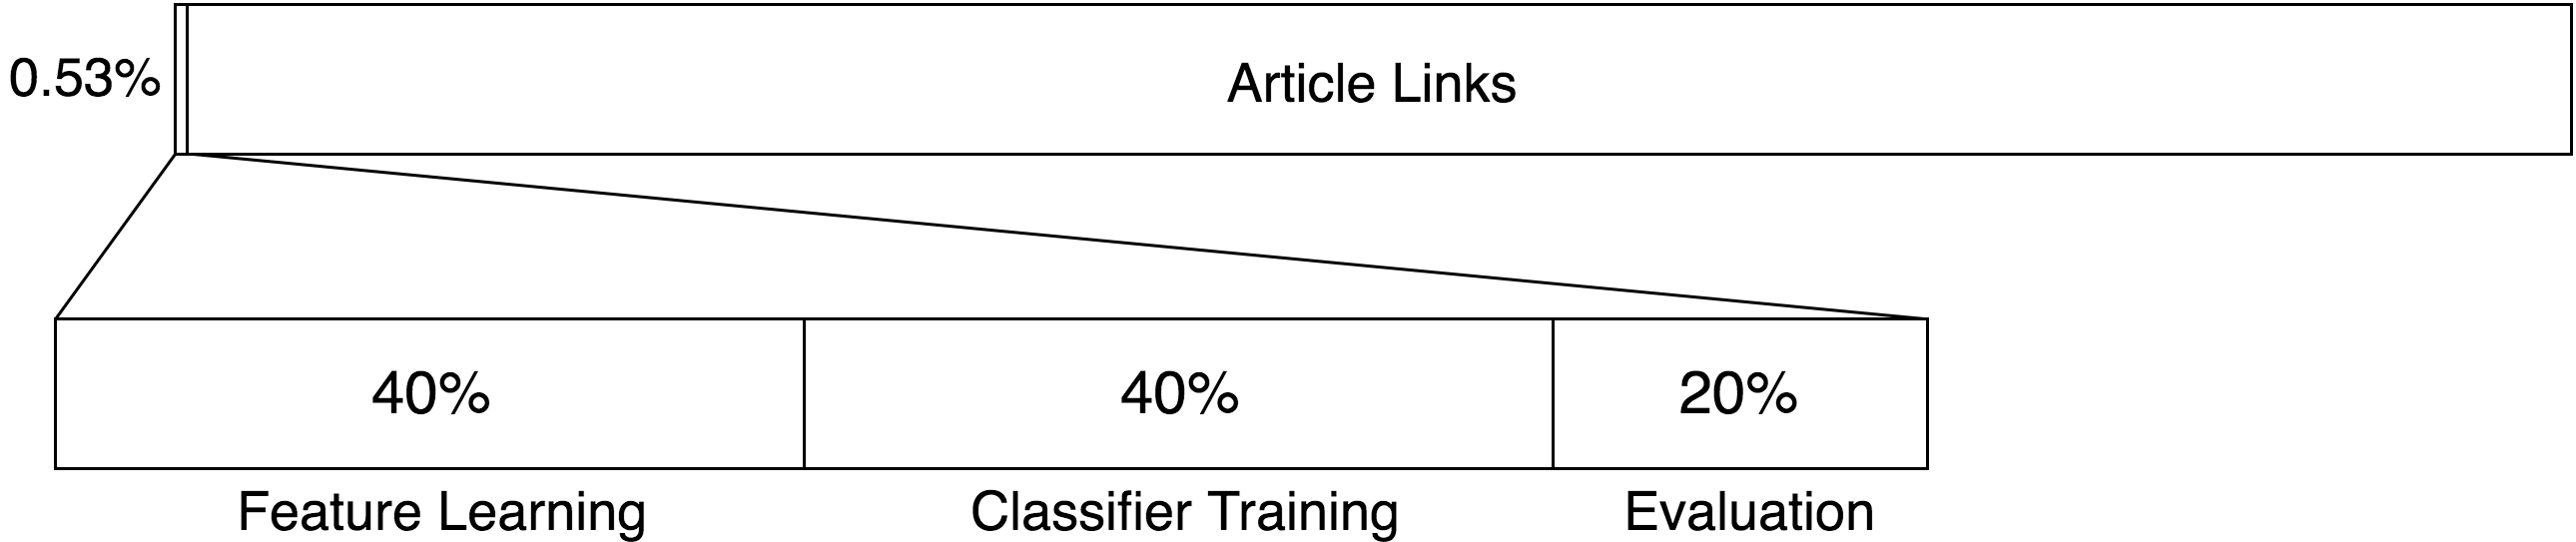
\includegraphics[width=\textwidth]{link-distribution}

\end{frame}
\note{
  \begin{itemize}
    \item Notes here...
  \end{itemize}
}


\begin{frame}
    \frametitle{Feature Learning}
    %\framesubtitle{Data Partitioning}
    \centering

    \begin{itemize}
      \item node2vec
      \item Article features
    \end{itemize}

    
\includegraphics[width=\textwidth]{feature-learning}

\end{frame}
\note{
  \begin{itemize}
    \item Notes here...
  \end{itemize}
}


\begin{frame}
    \frametitle{Feature Extraction}
    %\framesubtitle{Data Partitioning}
    \centering

    \begin{itemize}
      \item Combine article features using a non-commutative operation
    \end{itemize}

    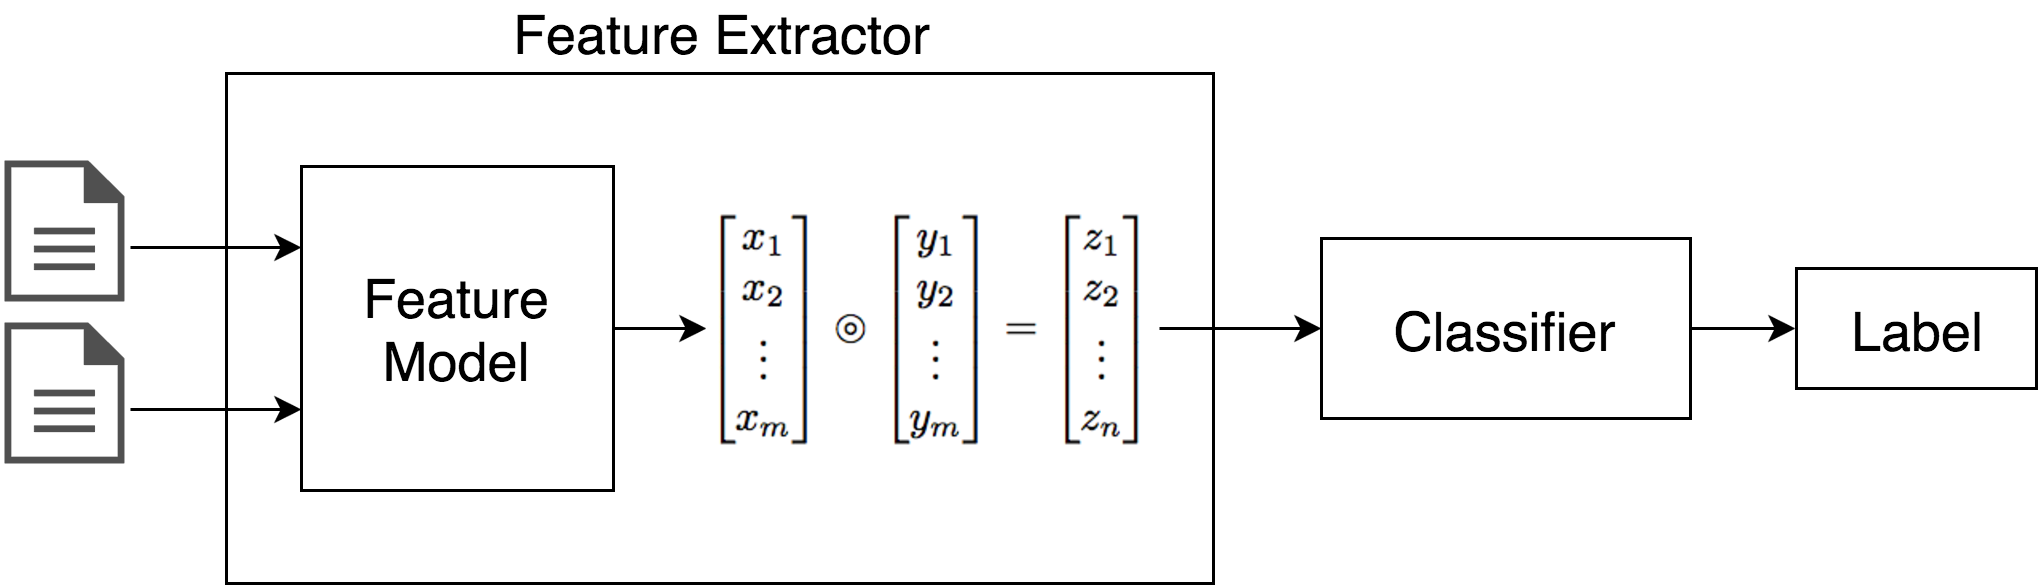
\includegraphics[width=\textwidth]{feature-extractor}

\end{frame}
\note{
  \begin{itemize}
    \item Notes here...
  \end{itemize}
}


\begin{frame}
    \frametitle{Classification}
    %\framesubtitle{Data Partitioning}
    \centering

    \begin{itemize}
      \item 10-fold cross-validation
    \end{itemize}

    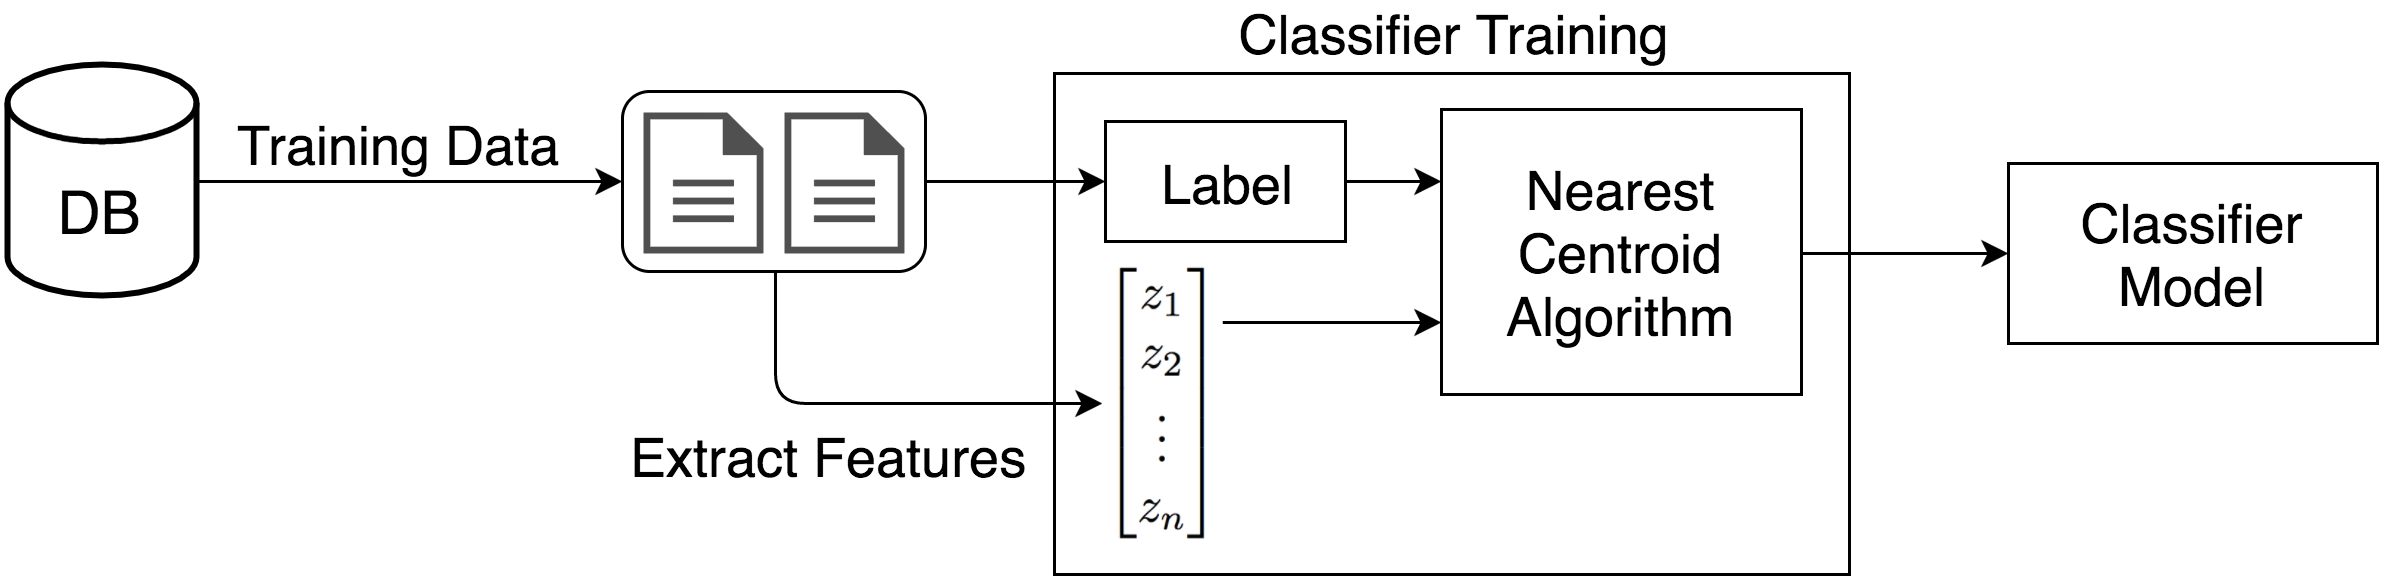
\includegraphics[width=\textwidth]{classifier-training}

\end{frame}
\note{
  \begin{itemize}
    \item Positive/Negative training samples
  \end{itemize}
}


\begin{frame}
    \frametitle{Pipeline}
    \framesubtitle{Components}
    \centering

    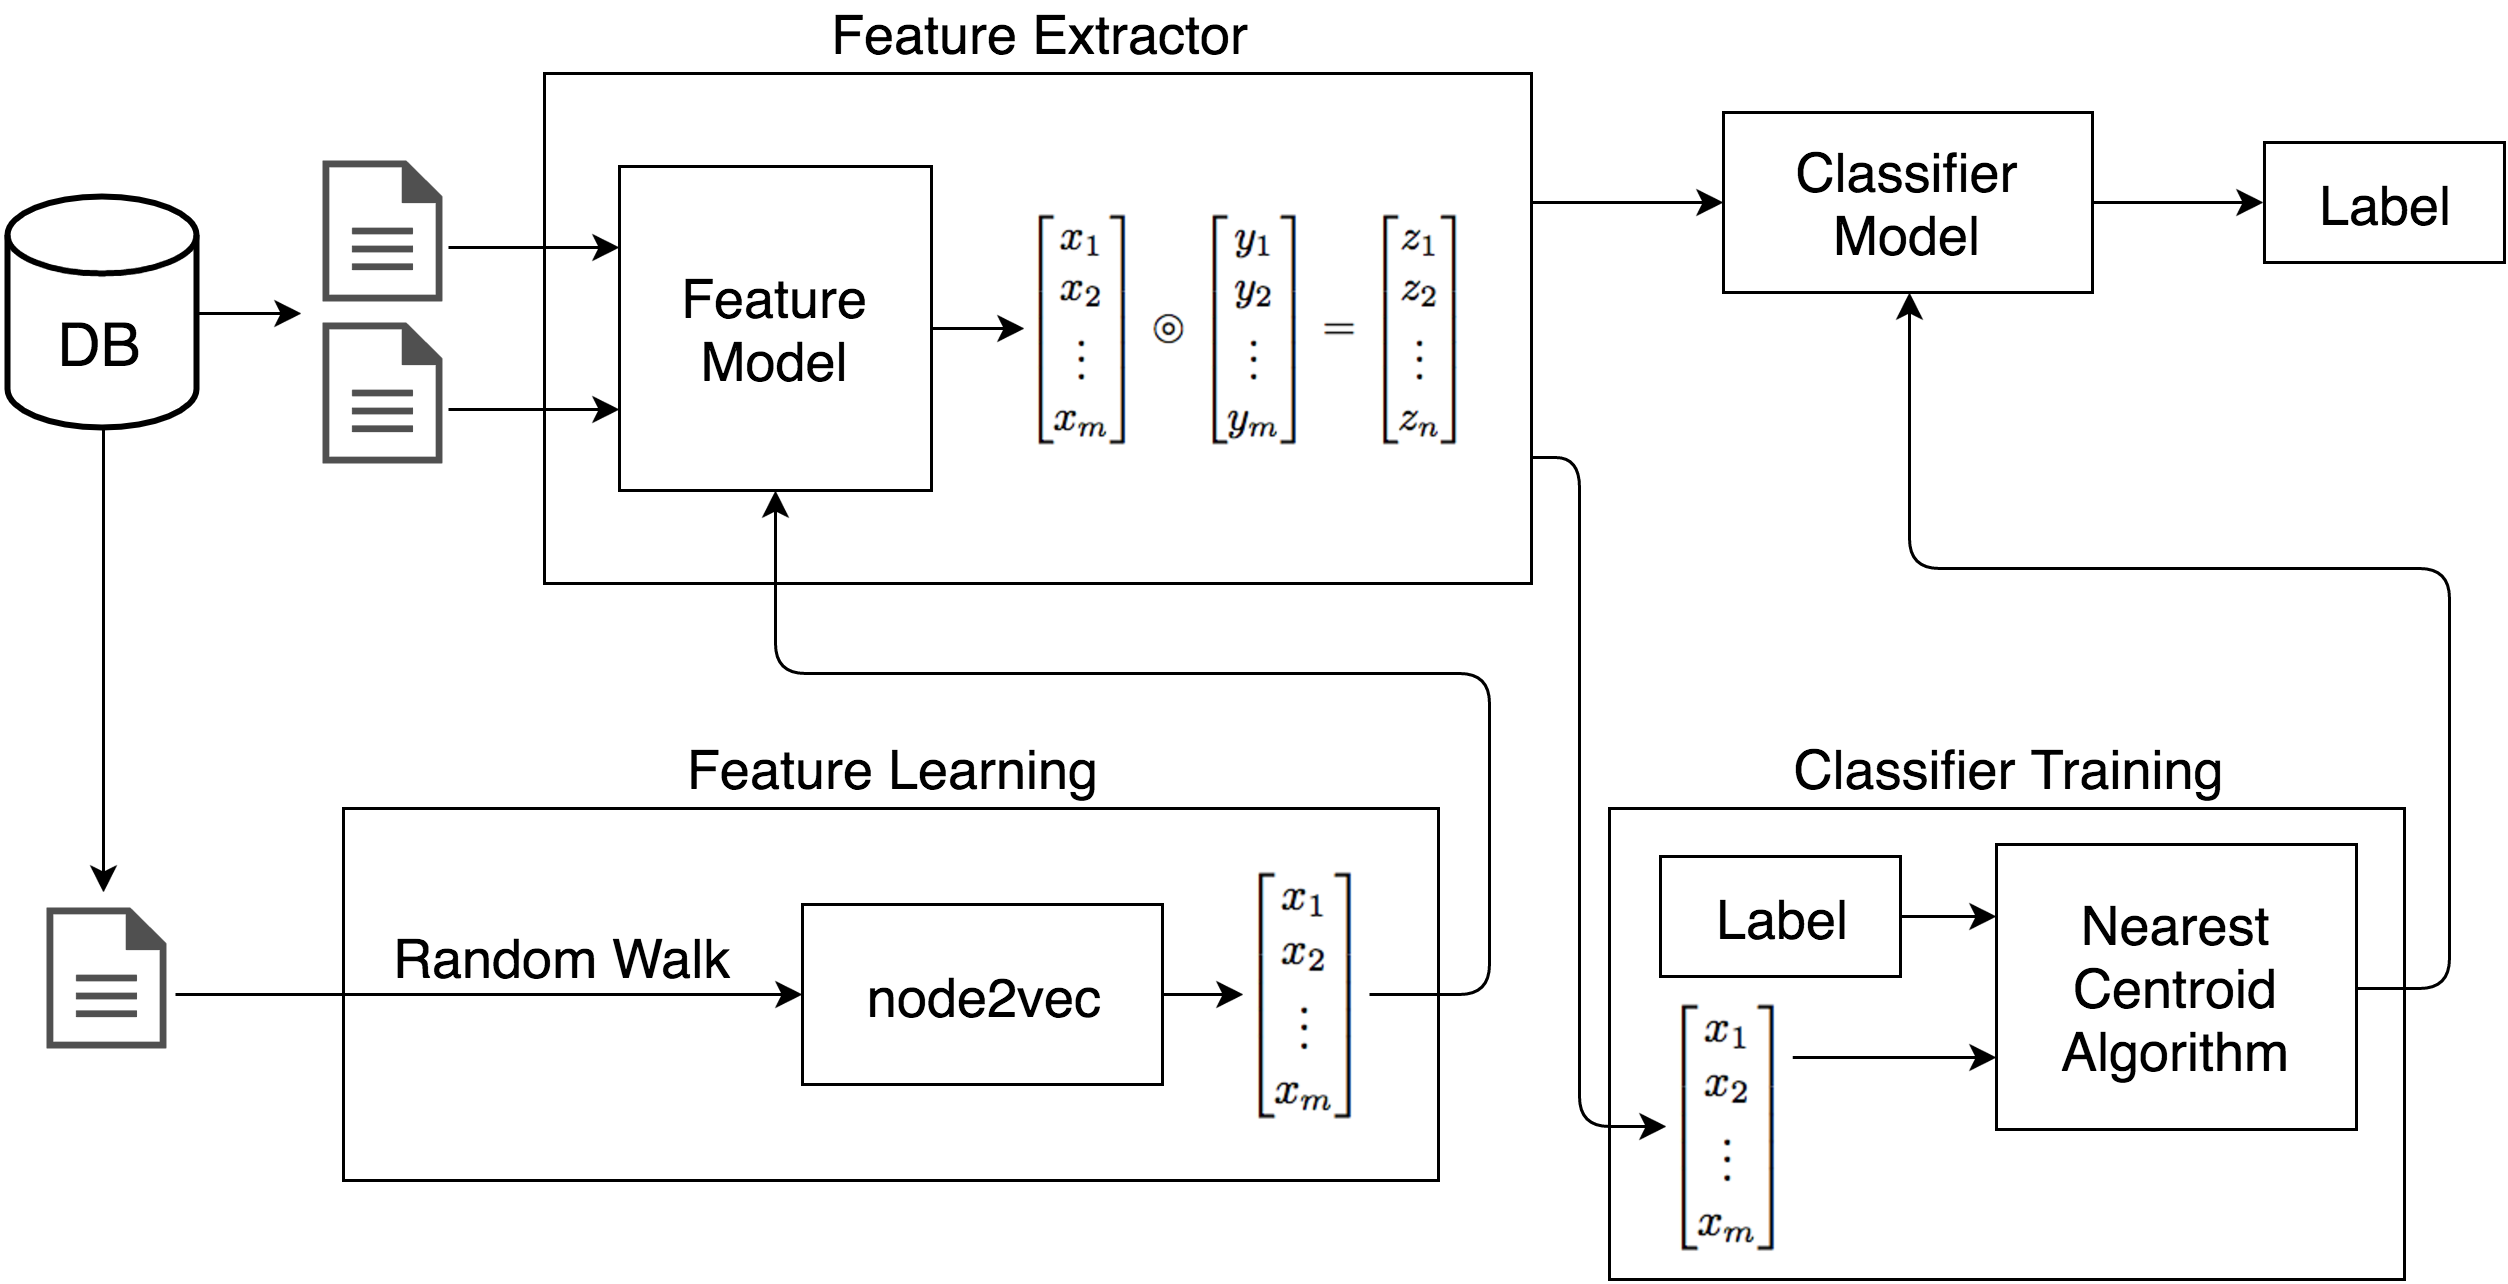
\includegraphics[width=\textwidth]{pipeline}

\end{frame}
\note{
  \begin{itemize}
    \item Online/Offline Learning
  \end{itemize}
}


